%!TEX root = ../iotpaper.tex

%~~~~~~~~~~~~~~~~~~~~~~~~~~~~~~~~~~~~~~~~~~~~~~~~~~~~~~~~~~~~~~~


\section{Gesture Library Experiments}
\label{sec:GestureLibrary}

\begin{table}

\begin{center}
  \begin{tabular}{ c | c | c | c  }
    \hline
    1 & 2 & 3 & 4  \\ \hline
    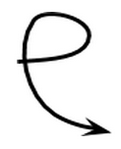
\includegraphics[width=0.2\linewidth, height=13mm]{./figures/gesture_e.png} & 
    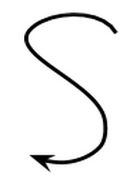
\includegraphics[width=0.2\linewidth, height=13mm]{./figures/gesture_s.png} &
    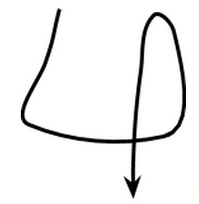
\includegraphics[width=0.2\linewidth, height=13mm]{./figures/gesture_num4.png} &
    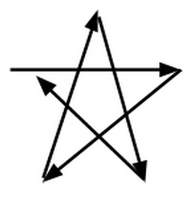
\includegraphics[width=0.2\linewidth, height=13mm]{./figures/gesture_star.png}  \\ \hline
    5 & 6 & 7 & 8 	 \\ \hline
    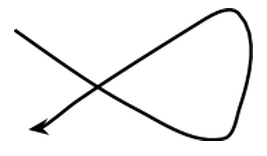
\includegraphics[width=0.2\linewidth, height=13mm]{./figures/gesture_5.png} &
    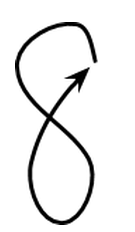
\includegraphics[width=0.2\linewidth, height=13mm]{./figures/gesture_num8.png} &
    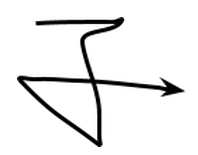
\includegraphics[width=0.2\linewidth, height=13mm]{./figures/gesture_7.png} &
    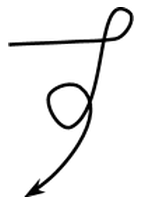
\includegraphics[width=0.2\linewidth, height=13mm]{./figures/gesture_su.png}  \\ \hline
    9 & 10 & 11 & 12  \\ \hline
    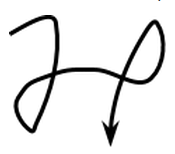
\includegraphics[width=0.2\linewidth, height=13mm]{./figures/gesture_mi.png} & 
    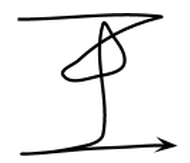
\includegraphics[width=0.2\linewidth, height=13mm]{./figures/gesture_wang.png} &
    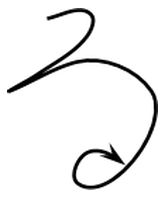
\includegraphics[width=0.2\linewidth, height=13mm]{./figures/gesture_ru.png} &
    
\includegraphics[width=0.2\linewidth, height=13mm]{./figures/gesture_miu.png}	\\ \hline
    13 & 14 & 15 & 16  \\ \hline
    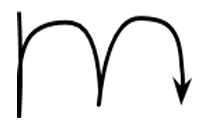
\includegraphics[width=0.2\linewidth, height=13mm]{./figures/gesture_m.png} &
    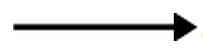
\includegraphics[width=0.2\linewidth, height=13mm]{./figures/gesture_14.png} &
    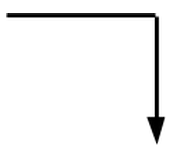
\includegraphics[width=0.2\linewidth, height=13mm]{./figures/gesture_15.png} & 
    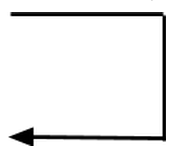
\includegraphics[width=0.2\linewidth, height=13mm]{./figures/gesture_16.png}  \\ \hline
    17    \\ \hline
    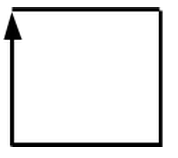
\includegraphics[width=0.2\linewidth, height=13mm]{./figures/gesture_17.png} \\ \hline
  \end{tabular}
\end{center}
\caption{The gestures used for testing authentication. This library is known for the Gesture Library model, and is unknown in the Simultaneous Gestures model.} % title of Table
\label{table:GestureTable}
\end{table}


To test the Gesture Library Model, we collect gesture data from all three group members. Our experimental library consists of the 17 different gestures shown in \autoref{tab:GestureTable}. These gestures are a mix of European characters, Asian characters, and simple shapes, each with varying complexity. 

Gino is the legitimate user who performed calibration on his iPhone 6 device. To emulate a strong attacker, Henry attempts authentication using a second iPhone 6 device. Joe is a weaker attacker who attempts authentication on an iPhone 6s. Joe is less familiar with Asian characters, and thus is weaker than Henry because of the selecting gestures. Gino also attempts authentication on his second device, the Nexus 5, as a legitimate user.

For each gesture, Gino takes 30 calibration attempts on his iPhone 6. Afterwards, everyone attempts 10 new authentications for each gesture each day. In the next sections, we discuss calibration and set thresholds that minimize false negatives (rejecting Gino, the legitimate user), while also minimizing false positives (accepting Henry or Joe, the attackers).

\subsection{Calibration Mechanism}

Our calibration mechanism is a brute force search that calculates the \gls{DTW} distance of one attempt time series to another for the same gesture. The calibrated time series selected is the attempt with the smallest average distance to all of the other attempts. This approach is non-scalable ($O(N^{2})$ where $N$ is the number of calibration attempts). However, scalability is not the focus of this project because we can make calibration a one-time event at the beginning and choose not to update the history for the purposes of this experiment. For calibration, we use the full 30 attempts per gesture data set unless otherwise noted.

\subsection{Gesture Distance Consistency}

\begin{figure}[!tb]
\centering
 \tikzdefaultformatgraph
%\resizebox{9cm}{!}{
   \input{../../Data/plots/SimilarityPlot_star.tikz}
%    }
   \caption{DTW distance for Gesture 4 for the Gesture Library Model. Error bars are the standard deviation.}
  \label{fig:RawDistanceStar}
\end{figure}

First, to prove that gesture-based authentication works, we monitor the consistency of the \gls{DTW} from the calibration time series over the period of 7 days for both the legitimate user and the attackers. We hypothesize that the average distance for all the attempts for a single gesture on a single day from the attackers stays at least one standard deviation away from the average distance for the intended user. 

\begin{figure}[!h]
\centering
 \tikzdefaultformatgraph
%\resizebox{9cm}{!}{
   \input{../../Data/plots/SimilarityPlot_su.tikz}
%    }
   \caption{DTW distance for Gesture 8 for the Gesture Library Model. Error bars are the standard deviation.}
  \label{fig:RawDistanceSu}
\end{figure}

\autoref{fig:RawDistanceStar} shows the typical distance for most gestures. The intended user (Gino's) raw \gls{DTW} is significantly lower than either of the attackers. However, \autoref{fig:RawDistanceSu} shows one of a few cases where one attacker (Henry) is able to match or get close to the distance of Gino, which invalidates our hypothesis. This typically happened on the first day, when Henry was able to see Gino do the gesture many times before authenticating himself. On other days, Henry and Joe did not see Gino calibrate and had to mimic based on memory. 

\subsection{Threshold Setting}
\label{subsec:thres}

\subsubsection{Technique}

The threshold for rejecting or accepting a user can be set using a variety of techniques. For this project, we use a simple threshold ($D_{t}$) based on the calibration data above as a proof of concept. Each attempt from calibration has an average \gls{DTW} distance from all of the other calibration attempts. Based on this distance, we can set a threshold tailored to gesture $i$ using \autoref{eq:thres}

\begin{equation}
D_{t} = m \cdot d_{i} + \frac{1.96 \cdot \delta_{i}}  {\sqrt{N}}
\label{eq:thres}
\end{equation}

\noindent where $m$ is a constant multiplicative factor, $d_{i}$ is a mean distance value based on the distance data from calibration for gesture $i$, and $\delta_{i}$ is the associated standard deviation.

Intuition suggests that choosing the minimum recorded \gls{DTW} distance for $d_{i}$ yields an overly strict system that minimizes false positives but also introduces additional false negatives to the system. Likewise, choosing the maximum recorded \gls{DTW} distance for $d_{i}$ produces an overly lenient system that minimizes false positives but introduces false negatives. 

To make the system more usable, we opt to split the difference to minimize both false positives and false negatives. However, if we must choose between more false positives and false negatives, we choose to err on the side of more false positives to make the system more usable to the end user. Therefore, we set $d_{i}$ based on the 80th, 85th, and 90th percentiles of the calibration data. This lets us minimize the effects of any major calibration outliers while still being lenient. Furthermore, the multiplicative factor $m$ is used to introduce some additional leniency because of day-to-day variation in the intended user's gesture. $m$ is varied from 1 to 5 in steps of 0.25.

Our hypothesis is that we can set an authentication distance threshold that keeps the false positives and false negatives rates averaged over all gestures below 10\% for all gestures.

\subsubsection{Results}

 \begin{figure*}[!t]
% 	\vspace{-1.5em}
    	\centering
 	\subfloat[80th Percentile]{
 	\centering
 	\tikzthirds
		\input{../../Data/plots/thresholdplots/threshold80thpercentile.tikz}
 		 \label{fig:80p}}
 	\subfloat[85th Percentile]{
 	\centering
 	\tikzthirds
		\input{../../Data/plots/thresholdplots/threshold85thpercentile.tikz}
 		 \label{fig:85p}}
 	\subfloat[90th Percentile]{
 	\centering
 	\tikzthirds
		\input{../../Data/plots/thresholdplots/threshold90thpercentile.tikz}
 		 \label{fig:90p}}
 	\caption{False positive and false negative results for various thresholds using various thresholds. Although the global minima for each percentile occurs at a lower multiplicative factor, we err on the side of less false negatives such that the intended user (Gino) finds it more usable.}
 	 \label{fig:ThresFig}
 \end{figure*}
 
The optimal threshold settings are the ones that minimize both the false positives and false negatives in \autoref{eq:thres}. \autoref{fig:ThresFig} shows the results for false positives and false negatives for the (a) 80th, (b) 85th, and (c) 90th percentiles. Based on these results, we can first conclude that our initial assessment of attacker strength is correct. Henry is a stronger attacker than Joe, so we focus on Henry and Gino for finding the best threshold. Next, we conclude that our hypothesis is invalidated because there exists no point there all false positives and false negatives are less than 10\%. Nonetheless, we next aim to see what is the best threshold multiplier and percentile setting that achieves the best performance. 

\begin{table}[!tb]
\begin{center}
  \begin{tabular}{| c | c | c | c | }
    \hline
    \emph{Percentile} & \emph{$m$} & \emph{False - (\%)} & \emph{False + (\%)}  \\ \hline \hline
    80 & 2.5 & 9.61 & 20.34 	 \\ \hline
    85 & 2.5 & 8.73 & 23.109 	 \\ \hline
    90 & 2.25 & 9.31 & 20.50 	 \\ \hline
  \end{tabular}
\end{center}
\caption{Best threshold settings that minimize false positives while keeping false negatives below 10\% where $m$ is the threshold multiplier.} % title of Table
\label{tab:FNFP}
\end{table}

The plots in \autoref{fig:ThresFig} show that the true minima lies between $m$ betwee 1.5 and 2.5 (roughly 15\% false positives and false negatives at the equilibrium point). When using the 80th percentile, $m$ is larger at the global minima than when using the other percentiles. This trend is because the thresholds are tighter when using a smaller percentile, so a larger multiplier is needed to compensate. 

However, we opt to prioritize getting the intended user's false negative rate to less than 10\%. For the percentiles shown above, this corresponds to the values shown in \autoref{tab:FNFP}. All of these settings show similar performance to each other, so any of these settings may be selected for such a system. 

%\subsection{Number of Calibration Iterations}
%
%Thus far, our evaluation is based on our full data set of 30 calibration attempts per gesture. In this section, we investigate the performance of our Gesture Library model for smaller subsets of calibration attempts: 5, 15, and 30. We hypothesize that we will have more false positives and false negatives for the same parameters because of the smaller data set.
%
%\hl{DATA HERE}.

\subsection{Multi-Challenge Authentication}

To address the high false positive rate observed in \autoref{subsec:thres}, we propose that multiple library gestures be used to challenge the prover during authentication instead of only selecting a single gesture. Our hypothesis is that, because the success ratio of the attacker (roughly 20-40\%) is much weaker than the success ratio of the user (roughly 90-95\%), there exists a number of challenges ($n_{c}$) such that false positives are reduced to less than 20\% while maintaining false negatives at less than 20\%. For evaluation purposes, we select the 80th percentile and select $m$ multipliers that yield various false negative ratios aggressively below 10\%. 

\begin{figure}[!t]
\centering
 \tikzdefaultformatgraph
%\resizebox{9cm}{!}{
   \input{../../Data/plots/multiauth.tikz}
%    }
   \caption{Probability of success for various multi-challenge authentication probabilities generated by the Gesture Library model.}
  \label{fig:multiauth}
\end{figure}

\autoref{fig:multiauth} shows the results for multi-challenge authentication. The curves indeed validate that the success probability drops off more quickly for the attacker than the prover for the smaller number of challenges. However, there is a diminishing return where adding more challenges trivially reduces false positives compared to the number of false negatives introduced. Using a FN rate fo 4.5\% and $n_{c}=2$ moves the equilibrium point from 15\% down to around 10\%. However, in order to get increasing returns from additional gesture challenges, the system requires an even more lenient system to reduce the false negative ratio even further.

%~~~~~~~~~~~~~~~~~~~~~~~~~~~~~~~~~~~~~~~~~~~~~~~~~~~~~~~~~~~~~~~
 

